\documentclass[a4paper,12pt]{article} 
\usepackage[utf8x]{inputenc}
\usepackage[french]{babel}
\usepackage{mathtools}
\usepackage{amsmath, amssymb, amsfonts}
\usepackage{textcomp}
\usepackage[nointegrals]{wasysym}			% Collection de symboles mathématiques
\usepackage{ifthen}
\usepackage{tabularx}	 				% Gestion avancée des tableaux
\usepackage{longtable}		
%\usepackage{cleveref}

\usepackage{mathrsfs}

\usepackage{enumitem}
\usepackage{wrapfig}
%\usepackage[squaren]{SIunits}
%\usepackage[T1]{fontenc}				% Indispendable, présent dans tous les codes exemples
\usepackage[linkcolor=Indigo, colorlinks=true, citecolor=DarkSlateBlue, urlcolor=MidnightBlue]{hyperref} 	% Hyper ref
\usepackage{listings}					% Pour citer du code
\usepackage[justification=centering]{caption}
\usepackage{sistyle} 
\usepackage{numprint}
\usepackage{wrapfig}
\usepackage{cite}	
\usepackage{url} 					% Pour citer les sites internet dans la
%\usepackage{cleveref}4
\usepackage{setspace}
\usepackage{graphicx}		 			% Inclusion des figures
\graphicspath{{./pic/}, {../figures/full_69_rapport/}}

\usepackage[svgnames]{xcolor}			%https://www.latextemplates.com/svgnames-colors

\title{\large{Licences SESI \& SESI/PEIP -- Semestre 1}}%%%%%%%%%%%%%%%%%%%%
\date{\large{18 Octobre 2018}}

%\usepackage{fancyhdr}
%\pagestyle{fancy}
%\fancyhead[RO]{\thepage}
%\fancyhead[RO]{}
%\lhead{
%\rhead{}
%\rhead{\markright}
\usepackage{geometry}
\geometry{hmargin=2.4cm, vmargin=3cm}

\usepackage{fancyhdr}
 
\pagestyle{fancy}
\fancyhf{}
\fancyhead[LE,RO]{Année 2018-2019}
\fancyhead[RE,LO]{ Université de Lille -- Faculté des Sciences et Technologies}

\begin{document}
\begin{center}
	\textbf{Licences SESI \& SESI/PEIP -- Semestre 1} \\[2mm]
	\large{\textbf{Bases de la Mécanique}} \\[1mm]
	\textit{Contrôle continu -- 18 Octobre 2018}
\end{center}
\begin{flushleft}
Aucun document ni appareil électronique autorisé \hfill Durée : 30 min
\end{flushleft}
\hrule
\vspace{2mm}
\subsection*{Questions de cours}
\begin{itemize}
\item[1)] Donner la définition du moment en K d'une force $\left( \vec{F}, A\right)$.
\item[2)] Écrire la relation de transport de ce moment en un point J quelconque et démontrer cette relation.
\item[3)] Énoncer le principe fondamentale de la statique.
\end{itemize}
\subsection*{Exercice}
Un avion léger est au repos sur le tarmac (Fig 1 et 2). On s'intéresse à l'équilibre de l'ensemble S formé de l'aile et de l'atterrisseur droits. On se donne un repère orthonormée de base $\left( \vec{x}, \vec{y}, \vec{z} \right)$.\\

\begin{figure}[!ht]
\centering
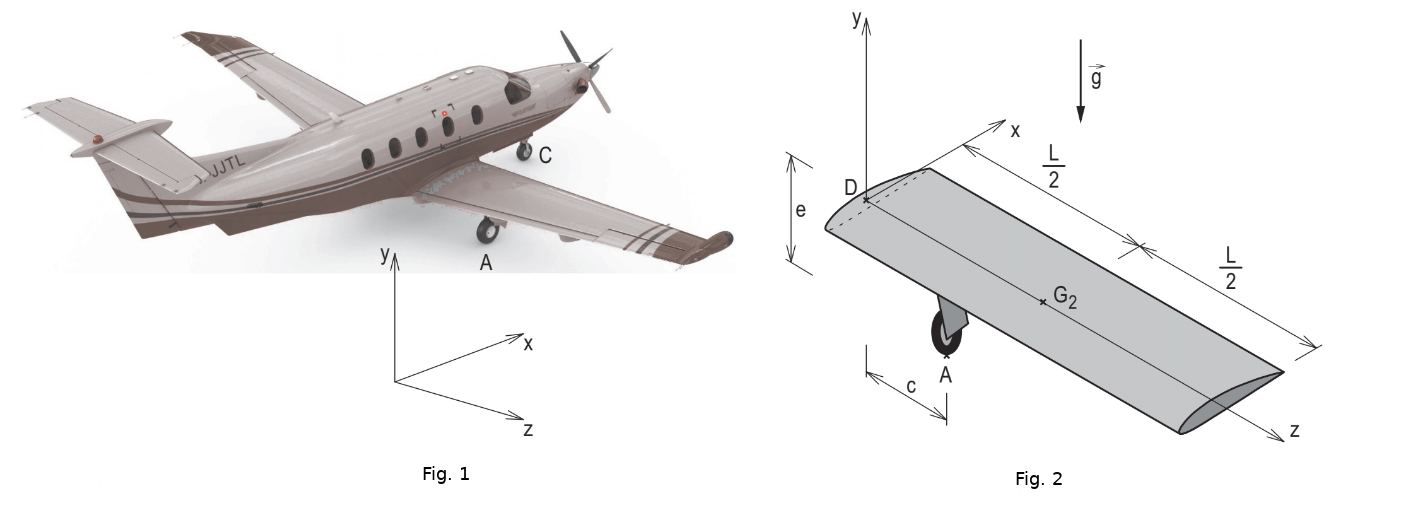
\includegraphics[scale=0.32]{pic_exo_statique.png}

\end{figure}

La modélisation de cet ensemble est donnée par la figure 2 et décrite ci-après :
\begin{itemize}[leftmargin=2cm]
	\item[--] La masse de cet ensemble est noté $m$, son centre de gravité $G_2$.
	\item[--] L'action du sol sur la roue est supposée \textbf{\textit{connue}} et s'écrit $\vec{R_A} = F_A \vec{y}$.
	\end{itemize}

Le contact en D n'est pas ponctuel et génère : \vspace{1mm}
	\begin{itemize}[leftmargin=2cm]
	\item[--] Une force $\vec{R_D} = D_y \vec{y} + D_z \vec{z}$
	\item[--] Un moment en D, $\vec{M}_D\left( \vec{R_D}, D\right) = M_D\, \vec{x}$ \textbf{\textit{non nul}}
	\end{itemize}

\begin{itemize}
\item[1)] Isoler le système S et effectuer un bilan des actions extérieures en précisant si les actions sont connues.\vspace{1mm}
\item[2)] Écrire ses équations vectorielles puis scalaires.\vspace{1mm}
\item[3)] En déduire les composantes de forces et de moment générées par le contact en D.  \vspace{2mm}
\end{itemize}
\hrule
\end{document}